% ######################################################################################################################
%         Supporting Information
% ######################################################################################################################

\chapter{Supporting Information}
\label{ch:SupportingInformation}

\begin{table}[htbp]
\caption[IUPAC notation of nucleobases and ambiguity characters]{
\textbf{IUPAC notation of nucleobases and ambiguity characters.}
The table lists the character representations of nucleobases and their combinations
(which are used to denote ambiguity) as suggested by the IUPAC Commission \cite{IUPAC1970}.
The names and symbols for ambiguity characters are chosen based on bio-chemical properties of the nucleobases.
See \secref{ch:Foundations:sec:SequenceAnalysis:sub:ConsensusSequences} for more information.
}
\label{tab:AmbiguityCharacters}
{
    \newcommand{\mc}[3]{\multicolumn{#1}{#2}{#3}}
    \newcommand{\rb}{\cellcolor{black!12}}
    \begin{center}
    \begin{tabular}{c|l|cccc|c|c}
%     \toprule
%     \hline
    Symbol & Description & \mc{5}{c|}{Represented Bases} & Complement \\
%     \midrule
    \hline
    A & \textbf{A}denine & \rb{} A &  &  &  & 1 & T \\
    C & \textbf{C}ytosine &  & \rb{} C &  &  & 1 & G \\
    G & \textbf{G}uanine &  &  & \rb{} G &  & 1 & C \\
    T & \textbf{T}hymine &  &  &  & \rb{} T & 1 & A \\
    U & \textbf{U}racil &  &  &  & \rb{} U & 1 & A \\
    \hline
    W & \textbf{W}eak & \rb{} A &  &  & \rb{} T & 2 & W \\
    S & \textbf{S}trong &  & \rb{} C & \rb{} G &  & 2 & S \\
    M & a\textbf{M}ino & \rb{} A & \rb{} C &  &  & 2 & K \\
    K & \textbf{K}eto &  &  & \rb{} G & \rb{} T & 2 & M \\
    R & pu\textbf{R}ine & \rb{} A &  & \rb{} G &  & 2 & Y \\
    Y & p\textbf{Y}rimidine &  & \rb{} C &  & \rb{} T & 2 & R \\
    \hline
    B & not A (\textbf{B} comes after A) &  & \rb{} C & \rb{} G & \rb{} T & 3 & V \\
    D & not C (\textbf{D} comes after C) & \rb{} A &  & \rb{} G & \rb{} T & 3 & H \\
    H & not G (\textbf{H} comes after G) & \rb{} A & \rb{} C &  & \rb{} T & 3 & D \\
    V & not T (\textbf{V} comes after T and U) & \rb{} A & \rb{} C & \rb{} G &  & 3 & B \\
    \hline
    N & any \textbf{N}ucleotide (not a gap) & \rb{} A & \rb{} C & \rb{} G & \rb{} T & 4 & N \\
    Z & \textbf{Z}ero &  &  &  &  & 0 &
%     \bottomrule
%     \hline
    \end{tabular}
    \end{center}
}
\end{table}

\begin{figure}[thb!p]
    \centering
    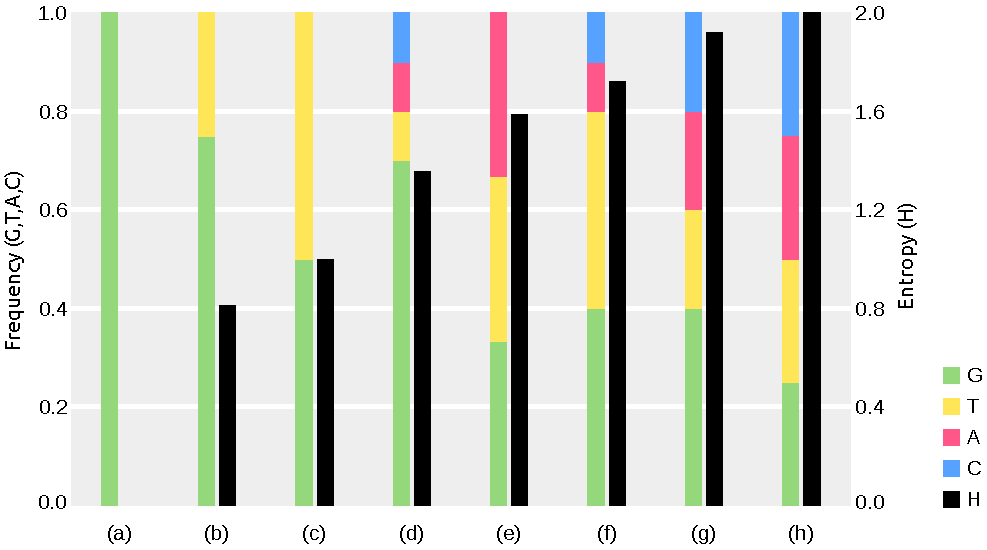
\includegraphics[width=\linewidth]{entropy.pdf}
    \begin{subfigure}{0pt}
        \phantomcaption
        \label{fig:entropy:sub:a}
    \end{subfigure}
    \begin{subfigure}{0pt}
        \phantomcaption
        \label{fig:entropy:sub:b}
    \end{subfigure}
    \begin{subfigure}{0pt}
        \phantomcaption
        \label{fig:entropy:sub:c}
    \end{subfigure}
    \begin{subfigure}{0pt}
        \phantomcaption
        \label{fig:entropy:sub:d}
    \end{subfigure}
    \begin{subfigure}{0pt}
        \phantomcaption
        \label{fig:entropy:sub:e}
    \end{subfigure}
    \begin{subfigure}{0pt}
        \phantomcaption
        \label{fig:entropy:sub:f}
    \end{subfigure}
    \begin{subfigure}{0pt}
        \phantomcaption
        \label{fig:entropy:sub:g}
    \end{subfigure}
    \begin{subfigure}{0pt}
        \phantomcaption
        \label{fig:entropy:sub:h}
    \end{subfigure}
    \caption[Examples of the per-site entropy for different character frequencies]{
        \textbf{Examples of the per-site entropy for different character frequencies.}
        The Figure shows the entropy $H$ that results from an alignment site with some exemplary nucleotide frequencies.
        See \secref{ch:AutomaticTrees:sec:Methods:sub:PhAT:par:SequenceEntropy}
        for details of the calculation of the per-site entropy,
        and for its application in the context of multiple sequence alignments.
        The entropy is symmetric with respect to permutations of the nucleobases;
        we here show examples using the nucleobase \nucleobase{G} as the most frequent character at the site.
        For simplicity, we here do not include the gap character.
        \\
        The subfigures are ordered by increasing entropy,
        which ranges from $0$ for a site with only a single character, as in \subref{fig:entropy:sub:a},
        to $2$ for a site with all four nucleobases equally frequent, as in \subref{fig:entropy:sub:h}.
%         \subref{fig:entropy:sub:a} The site only contains one character, the resulting entropy is $0$.
%         \subref{fig:entropy:sub:b}, \subref{fig:entropy:sub:c} Another character appears with 25\% and 50\% frequency, respectively.
%         \subref{fig:entropy:sub:d} One character appears with 70\% frequency, the three remaining ones with 10\% each.
%         \subref{fig:entropy:sub:e} Three characters with equal frequency of 33.3\% each.
%         \subref{fig:entropy:sub:f} Two characters with 40\%, and two with 10\% frequency.
%         \subref{fig:entropy:sub:g} One character with 40\%, and three with 20\% frequency each.
%         \subref{fig:entropy:sub:h} All four characters are equally frequent with 25\% each, resulting in the maximum entropy of $2$.
        The maximum possible entropy is given by the base of the logarithm.
        The choice of base is irrelevant when comparing entropies with each other,
        as it simply introduces a constant factor.
    }
    \label{fig:entropy}
\end{figure}


% ######################################################################################################################
%         Empirical Datasets
% ######################################################################################################################

\chapter{Empirical Datasets}
\label{ch:EmpiricalDatasets}

\paperbox{
    This chapter is partially based on the peer-reviewed publications:
}{\paperart \paperpppp}{
    \textbf{Contributions:} Lucas Czech... Alexandros Stamatakis...
}

We used three % four
% Neptrops got kicked out. One result of the neotrop paper was that the sequences are hyper diverse, so no good clusters.
% Furthermore, there is not much meta-data. So not a good dataset for either of the methods...
real world datasets to evaluate our methods:

\begin{itemize}
    \item   \acf{BV} \cite{Srinivasan2012}.
            This small dataset was already analyzed with phylogenetic placement in the original publication.
            We used it as an example of an established study to compare our results to.
            It has \num{220} samples with a total of \num{15 060} unique sequences.
    \item   \acf{NTS} \cite{Mahe2017}.
            \todo{check}
            We already analyzed this medium-sized dataset in its publication and found that
            the sequences are highly diverse and not well covered in existing reference databases.
            This was a particular challenge for classical approaches for metagenomic studies.
            It is thus used as an example of a difficult dataset here.
            It contains \num{154} samples with \num{10 567 804} unique sequences in total.
    \item   \acf{TO} \cite{Karsenti2011,Sunagawa2015,Guidi2016}.
            This world-wide sequencing effort of the open oceans provides a rich set of meta-data,
            such as geographic location, temperature, and salinity.
            Unfortunately, the sample analysis for creating the official data repository is still ongoing.
            % See https://www.embl.de/tara-oceans/start/research/index.html
            We thus were only able to use \num{370} samples with \num{27 697 007} unique sequences.
    \item   \acf{HMP} \cite{Huttenhower2012,Methe2012}.
            This large data repository intends to characterize the human microbiota.
            It contains \num{9192} samples from different body sites with a total of \num{63 221 538} unique sequences.
            There is additional meta-data such as age and medical history, which is available upon special request.
            We only used the publicly available meta-data.
    \item   \todo{mouse gut}
\end{itemize}

Details of the datasets (download links, data statistics, data preprocessing, etc.)
are provided in \todo{S1 Text}. %Supplementary Section \nameref{supp:sec:DetailsEmpiricalDatasets}.
At the time of writing, about one year after we initially downloaded the data,
the \ac{TO} repository has grown to \num{1 170} samples,
while the \ac{HMP} even published a second phase and now comprises \num{23 666} samples of the 16S region.
This further emphasizes the need for scalable methods to analyze such data.

These datasets represent a wide range of environments, number of samples, and sequence lengths.
We use them to evaluate our methods and to exemplify which method is applicable to what kind of data.
To this end, the sequences of the datasets were placed on appropriate phylogenetic \acp{RT} as explained
in \todo{S1 Text}, in order to obtain phylogenetic placements that our methods can be applied to.
In the following, we present the respective results, and also compare our methods to other methods
where applicable.
As the amount and type of available meta-data differs for each dataset,
we could not apply all methods to all datasets.
Lastly, we also report the run-time performance of our methods on these data.

The analyses and figures presented here were conducted on distinct reference alignments and trees.
Firstly, for the \ac{BV} dataset, we used the original set of reference sequences, and re-inferred a tree on them.
Secondly, for the \ac{TO} and \ac{HMP} datasets, we used our Phylogenetic Automatic (Reference) Tree \ac{PhAT} method \cite{Czech2018}
to construct sets of suitable reference sequences from the \toolname{Silva} database \cite{Quast2013,Yilmaz2014}.
We used the 90\% threshold consensus sequences;
see \cite{Czech2018} for details.

For all analyses, we used the following software setup:
Unconstrained maximum likelihood trees were inferred using \toolname{RAxML v8.2.8} \cite{Stamatakis2014}.
% Didn't use any constrained trees in this paper. Thus, don't need the following:
% Constrained trees were inferred with \toolname{Sativa 0.9-55} \cite{Kozlov2016},
% which internally again relies on \toolname{RAxML},
% and offers a convenient way to turn a taxonomy into a constraint tree.
For aligning reads against reference alignments and reference trees,
we used a custom MPI wrapper for \toolname{PaPaRa 2.0} \cite{Berger2011a,Berger2012},
which is available at \cite{PaPaRaMPI}.
We then applied the \texttt{chunkify} procedure as explained in \cite{Czech2018}
to split the sequences into chunks of unique sequences prior to conducting the phylogenetic placement,
in order to minimize processing time.
Phylogenetic placement was conducted using \toolname{EPA-ng} \cite{Barbera2018},
which is a faster and more scalable phylogenetic placement implementation
than \toolname{RAxML-EPA} \cite{Berger2011} and \toolname{pplacer} \cite{Matsen2010}.
Lastly, given the per-chunk placement files produced by \toolname{EPA-ng}, we executed the \texttt{unchunkify} procedure of \cite{Czech2018}
to obtain per-sample placement files. These subsequently served as the input data for the methods presented here.

\begin{table}[htb]
\caption[Overview of the dataset dimensions]{
\textbf{Overview of the dataset dimensions.}
The ``Samples'' columns show how many metagenomic samples there were in the originally downloaded data and
how many of those we actually used for our experiments after filtering out spurious ones.
The columns ``Filtered Sample Sizes'' show how many sequences each of the filtered samples has.
The ``Sequence Count'' columns show the total number of sequences in the filtered samples, and how many of them are unique.
The columns ``Sequence Length'' show statistics of the length of the sequences.
Lastly, the ``Chunks'' column shows into how many chunks of size \num{50 000} the samples were distributed.
}
\label{tab:MetagenomicDatasetsOverview}
{
    \newcommand{\mc}[3]{\multicolumn{#1}{#2}{#3}}
    \begin{center}
    \begin{tabular}{l|rr|rrr|rr|rrr|r}
                        & \mc{2}{c|}{Samples}                      & \mc{3}{c|}{Filtered Sample Sizes}                 & \mc{2}{c|}{Filtered Sequence Count}   & \mc{3}{c|}{Filtered Sequence Length}              & \mc{1}{r}{} \\
    Dataset             & \mc{1}{r}{Source} & \mc{1}{r|}{Filtered} & \mc{1}{r}{Min} & \mc{1}{r}{Max} & \mc{1}{r|}{Avg} & \mc{1}{r}{Total} & \mc{1}{r|}{Unique} & \mc{1}{r}{Min} & \mc{1}{r}{Max} & \mc{1}{r|}{Avg} & Chunks \\
    \hline
    Bacterial Vaginosis &                   &                  220 &                &                &                 &          426,612 &             15,060 &                &                &             226 &      1 \\
    Neotropical Soils   &                   &                  154 &                &                &                 &       50,118,536 &         10,567,804 &                &                &             364 &    212 \\
    Tara Oceans         &                   &                  370 &                &                &                 &       49,023,231 &         27,697,007 &                &                &             128 &    554 \\
    Human Microbiome    &             9,815 &                9,194 &                &                &                 &      118,701,818 &         63,221,538 &                &                &             413 &  1,265 \\
    \end{tabular}
    \end{center}
}
\end{table}

% ======================================================================================================================
%     Bacterial Vaginosis
% ======================================================================================================================

\section{Bacterial Vaginosis}
\label{supp:sec:DetailsEmpiricalDatasets:sub:BV}

We used the Bacterial Vaginosis dataset \cite{Srinivasan2012} in order to compare our novel methods to
existing ones such as Edge PCA and Squash Clustering \cite{Matsen2011a,Evans2012}.
The dataset contains metabarcoding sequences of the vaginal microbiome of \num{220} women,
and was kindly provided by Sujatha Srinivasan.
This small dataset with a total of \num{426 612} query sequences, thereof \num{15 060} unique,
was already analyzed with phylogenetic placement methods in the original publication.
We re-inferred the reference tree of the original publication using the original alignment,
which contains \num{797} reference sequences specifically selected to represent the vaginal microbiome.
As the query sequences were already prepared,
no further preprocessing was applied prior to phylogenetic placement.
The available per-sample quantitative meta-data for this dataset comprises
the Nugent score \cite{Nugent1991}, the value of Amsel's criteria \cite{Amsel1983}, and the vaginal pH value.
We used all three meta-data types in our analyses.

\todo{ from art: }

For testing the accuracy of our unconstrained \taxonname{Bacteria} tree on real data,
we used a vaginal microbiome dataset of 220 women \citep{Srinivasan2012},
which was provided by Sujatha Srinivasan.
See \figref{fig:bv_squash} and \figref{fig:bv_edgepca} for the respective results.
This small dataset with a total of \num{426 612} query sequences, thereof \num{15 060} unique,
was already analyzed with phylogenetic placement methods in the original publication.
We used it as an example of a well-designed study to assess our results using an \ac{PhAT} as reference tree.
In addition to the \taxonname{Bacteria} \ac{PhAT},
we re-inferred the reference tree of the original publication using their alignment,
again using \toolname{RAxML~8.2.8} \citep{Stamatakis2014}.
The query sequences of the dataset were then aligned to our reference tree and alignment,
as well as to the reference alignment of the original publication and our re-inferred tree.
For aligning, we used a custom MPI wrapper of \toolname{PaPaRa~2.0} \citep{Berger2011a,Berger2012},
which is available at \citep{PaPaRaMPI}.
Finally, the query sequences were placed on these trees using \toolname{EPA-ng} \citep{Barbera2018},
and the analyses were subsequently performed as explained in \figref{fig:bv_squash} and \figref{fig:bv_edgepca}.
\todo{the above is not up to date!}

% ======================================================================================================================
%     Neotropical Soils
% ======================================================================================================================

\section{Neotropical Soils}
\label{supp:sec:DetailsEmpiricalDatasets:sub:NTS}

% ======================================================================================================================
%     Tara Oceans
% ======================================================================================================================

\section{Tara Oceans}
\label{supp:sec:DetailsEmpiricalDatasets:sub:Tara}

The \acf{TO} dataset \cite{Karsenti2011,Sunagawa2015,Guidi2016}
that we used here contains amplicon sequences of protists,
and is available at \url{https://www.ebi.ac.uk/ena/data/view/PRJEB6610}.
% Seawater was filtered from different depths to retain small and large cell sizes (Protists Organisms).
% The DNA was extracted and amplified by PCR.
At the time of download, there were \num{370} samples available
with a total of \num{49 023 231} sequences.
As the available data are raw \texttt{fastq} files,
we followed \cite{FredsMetabarcodingPipeline} to generate cleaned per-sample \texttt{fasta} files.
For this, we used our tool \toolname{PEAR} \cite{Zhang2014} to merge the paired-end reads;
\toolname{cutadapt} \cite{Martin2011} for trimming tags as well as forward and reverse primers;
and \toolname{vsearch} \cite{Rognes2016} for filtering erroneous sequences and
generating per-sample \texttt{fasta} files.
We filtered out sequences below \SI{95}{bps} and above \SI{150}{bps}, to remove potentially erroneous sequences.
No further preprocessing (such as chimera detection) was applied.
This resulted in a total of \num{48 036 019} sequences, thereof \num{27 697 007} unique.
The sequences were then used for phylogenetic placement as explained above.
We placed the sequences on the unconstrained \taxonname{Eukaryota} reference tree obtained via our \ac{PhAT} method \cite{Czech2018},
which comprises \num{2 059} taxa, thereof \num{1 795} eukaryotic sequences.
The remaining \num{264} taxa are \taxonname{Archaea} and \taxonname{Bacteria},
and were included as a broad outgroup.
The \ac{TO} dataset has a rich variety of per-sample meta-data features;
in the context of this paper, we mainly focus on quantitative features such as
temperature, salinity, as well as oxygen, nitrate and chlorophyll content of the water.
Furthermore, each sample has meta-data features indicating the date, longitude and latitude, depth, etc.~of the sampling location.
This data might be interesting for further correlation analyses based on geographical information.
We did not use them here, as for example longitude and latitude would require a more involved method
that also accounts for, e.g., ocean currents.
Furthermore, geographical coordinates yield pairwise distances between samples,
which are not readily usable with our correlation analysis.
Lastly, in order to use features such as the date, that is, in order to analyze samples over time,
the same sampling locations would need to be visited at different times during the year,
which is not the case for the Tara Oceans expedition.

% ======================================================================================================================
%     Human Microbiome Project
% ======================================================================================================================

\section{Human Microbiome Project}
\label{supp:sec:DetailsEmpiricalDatasets:sub:HMP}

We used the \acf{HMP} dataset \cite{Huttenhower2012,Methe2012} for testing the scalability of our methods.
In particular, we used the ``HM16STR'' data of the initial phase ``HMP1'',
which are available from \url{http://www.hmpdacc.org/hmp/}.
The dataset consists of trimmed 16S rRNA sequences of the \texttt{V1V3}, \texttt{V3V5}, and \texttt{V6V9} regions.
The data are further divided into a ``by\_sample'' set and a ``healthy'' set,
which we merged in order to obtain one large dataset, with a total of \num{9 811} samples.
We then removed \num{10} samples that were larger than \SI{70}{\mega\byte}
as well as \num{605} samples that had fewer than \num{1 500} sequences,
because we considered them as defective or unreliable outliers.
% because they lack enough detail for properly measuring the KR distance,
Finally, we also removed \num{2} samples that did not have a valid body site label assigned to them.
This resulted in a set of \num{9192} samples
containing a total of \num{118 702 967} sequences with an average length of \SI{413}{bps}.
From these samples, sequences with a length of less than \SI{150}{bps}
as well as sequences longer than \SI{540}{bps} were removed,
as we considered them potentially erroneous.
No further preprocessing (such as chimera detection) was applied.
This resulted in a total of \num{116 520 289} sequences, of which \num{63 221 538} were unique.
We then used the unconstrained \taxonname{Bacteria} tree of our \ac{PhAT} method \cite{Czech2018} for phylogenetic placement.
The tree comprises \num{1 914} taxa, thereof \num{1 797} bacterial sequences.
The remaining \num{117} taxa are \taxonname{Archaea} and \taxonname{Eukaryota},
and were included as a broad outgroup.
Each sample is labeled with one of \num{18} human body site locations where it was sampled.
This is the only publicly available meta-data feature.
% See Table~\ref{tab:hmp_data_overview} for an overview of those labels.

\todo{ from art: }

We used the \acf{HMP} dataset \citep{Huttenhower2012,Methe2012} for further testing our methods
(see Figure~\ref{fig:hmp_mds_epca}).
In particular, we used the ``HM16STR'' data of their initial phase ``HMP1'',
which are available from \url{http://www.hmpdacc.org/hmp/}.
The dataset consists of trimmed 16S rRNA sequences of the \texttt{V1V3}, \texttt{V3V5}, and \texttt{V6V9} regions.
Each sample of the dataset is labeled with the human body site where it was obtained.
See Table~\ref{tab:hmp_data_overview} for an overview of those labels.
The data are further divided into a ``by\_sample'' set and a ``healthy'' set,
which we merged in order to obtain one large dataset, with a total of \num{9 811} samples.
We then removed \num{10} samples that were larger than \SI{70}{\mega\byte}
as well as \num{605} samples that had fewer than \num{1 500} sequences,
because we considered them as outliers,
% because they lack enough detail for properly measuring the KR distance,
and finally \num{2} samples that did not have a valid body site label assigned to them.
This resulted in a set of \num{9192} samples
containing a total of \num{118 702 967} sequences with an average length of \SI{413}{bps}.
From these samples, sequences with a length less than \SI{150}{bps}
as well as sequences longer than \SI{540}{bps} were removed.
No further preprocessing (e.g., chimera detection) was applied.
This resulted in a total of \num{116 520 289} sequences, of which \num{63 221 538} were unique.
These were split into \num{1 265} chunks of size \num{50 000} each, which were subsequently aligned to and
placed on the unconstrained \taxonname{Bacteria} tree with \num{2 059} tips using the steps explained above.
The chunk placements were then transformed again into per-sample placement files,
before finally running the steps explained in Figure~\ref{fig:hmp_mds_epca}.
% see mapseq paper for another example of hmp processing description

% --------------------------------------------
%     HMP Dataset Labels
% --------------------------------------------

\begin{table}[htb]
\caption[HMP Dataset Overview]{
\textbf{HMP Dataset Overview.}
The table lists the \num{18} body site labels used by the Human Microbiome Project (HMP) \citep{Huttenhower2012,Methe2012},
and a ``translation'' into the corresponding body region.
We used this dataset to evaluate the applicability of typical analysis methods for phylogenetic placement
using our \acp{PhAT}, see \secref{ch:AutomaticTrees:sec:Evaluation:sub:EmpiricalDatasets:par:HMP} for details.
Furthermore, we evaluated our $k$-means clustering methods on this dataset,
as described in \secref{ch:Clustering:sec:Results:sub:HMPDataset}.
% In order to simplify the visualization in \figref{fig:hmp_mds_epca},
In these evaluations,
we summarized some of the labels into eight location groups, as shown in the third column.
The last column lists how many samples from each body site were used in our evaluation.
}
\label{tab:hmp_data_overview}
{
    \begin{center}
    \begin{tabular}{lllr}
        \toprule
        Body Site                       & Region            & Group             & Samples   \\
        \midrule
        Stool                           & Stool             & Stool             & 600   \\
        Saliva                          & Saliva            & Saliva            & 529   \\
        Tongue Dorsum                   & Mouth (back)      & Mouth (back)      & 610   \\
        Throat                          & Mouth (back)      & Mouth (back)      & 638   \\
        Palatine Tonsils                & Mouth (back)      & Mouth (back)      & 599   \\
        Attached Keratinized Gingiva    & Mouth (front)     & Mouth (front)     & 600   \\
        Hard Palate                     & Mouth (front)     & Mouth (front)     & 566   \\
        Buccal Mucosa                   & Mouth (front)     & Mouth (front)     & 597   \\
        Subgingival Plaque              & Plaque            & Plaque            & 595   \\
        Supragingival Plaque            & Plaque            & Plaque            & 608   \\
        Anterior Nares                  & Nose              & Airways           & 541   \\
        Left Antecubital Fossa          & Arm               & Skin              & 290   \\
        Right Antecubital Fossa         & Arm               & Skin              & 328   \\
        Left Retroauricular Crease      & Ear               & Skin              & 596   \\
        Right Retroauricular Crease     & Ear               & Skin              & 604   \\
        Vaginal Introitus               & Vagina            & Vagina            & 292   \\
        Mid Vagina                      & Vagina            & Vagina            & 298   \\
        Posterior Fornix                & Vagina            & Vagina            & 301   \\
%         N/A                             &                   &                   & 2     \\
        Sum                             &                   &                   & 9192  \\
        \bottomrule
    \end{tabular}
    \end{center}
}
\end{table}

% ======================================================================================================================
%     Mouse Gut
% ======================================================================================================================

\section{Mouse Gut}
\label{supp:sec:DetailsEmpiricalDatasets:sub:MouseGut}

This dataset was used for the eval of tax assign in \secref{ch:AutomaticTrees:sec:Evaluation:sub:TaxonomicAssignmentProfiling}

CAMI Challenge \citep{Sczyrba2017}.
The CAMI Challenge is a community-driven effort to assess taxonomic profiling methods
using a common set of benchmark data sets.


we utilized the \taxonname{mouse gut} data set of the 2nd CAMI Challenge \citep{Bremges2018}.


More specifically, we used the unpaired HiSeq reads of the mouse gut data set from CAMI,
which comprises \num{64} samples of simulated reads.
The preprocessing involved read de-interleaving following \cite{DeinterleaveFastq},
paired-end read merging using \toolname{PEAR} \citep{Zhang2014},
as well as quality filtering and conversion to \texttt{fasta} using \toolname{VSEARCH2} \citep{Rognes2016}.
This yielded a total of \num{800 341 409} reads.
As our trees are based on small ribosomal subunit sequences,
we also performed read filtering to obtain reads from the 16S rDNA region
(see \secref{ch:Foundations:sec:SequenceAnalysis:sub:Metagenomics}).
This filtering was performed using the protocol of \cite{Logares2014},
which relies on \toolname{HMMER} \citep{Eddy1998,Eddy2009}, and respective profiles for the 16S rDNA locus.
We performed a global identity based de-replication step on the resulting reads that yielded \num{616 405} query sequences.
We aligned these query sequences to our \taxonname{Bacteria} reference alignment
using \toolname{PaPaRa~2.0} \citep{Berger2011a,Berger2012}.
We then performed phylogenetic placement of the aligned query sequences onto the unconstrained and constrained reference trees,
respectively, using \toolname{EPA-ng} \citep{Barbera2018}.
We performed de-de-replication to obtain per-sample data again, %on the \texttt{jplace} file,
resulting in \num{64} \texttt{jplace} files (one per original sample) with placements of the 16S rDNA sequences,
for each of the two trees.


Finally, we performed taxonomic assignment and taxonomic profiling of the per-sample results
using the \texttt{assign} command implemented in \toolname{gappa},
which works analogously to the method used in \toolname{Sativa} \citep{Kozlov2016}.
Its basic steps are described in \appref{ch:PipelineImplementation}.


% ######################################################################################################################
%         Pipeline and Implementation
% ######################################################################################################################

\cleardoublepage

\chapter{Pipeline and Implementation}
\label{ch:PipelineImplementation}

\paperbox{
    This chapter is based on the peer-reviewed publications:
}{\paperart \paperpppp}{
    \textbf{Contributions:} Lucas Czech... Alexandros Stamatakis...
}

\todo{add genesis and gappa logos. because we can.}

The methods described here are implemented in our tool \toolname{gappa},
which is freely available under GPLv3 at \url{http://github.com/lczech/gappa}.
\toolname{gappa} internally uses our C++ library \toolname{genesis},
which offers functionality for working with phylogenies and phylogenetic placement data,
and also contains methods to work with taxonomies, sequences and many other data types.
\toolname{genesis} is also freely available under GPLv3 at \url{http://github.com/lczech/genesis}.

\toolname{gappa} offers a command line interface for conducting typical tasks when working with phylogenetic placements.
The methods that we described here are implemented via the following sub-commands:

\begin{itemize}
    \item \texttt{dispersion}: The command takes a set of jplace files (called samples), and calculates and visualizes
        the Edge Dispersion per edge of the reference tree.
    \item \texttt{correlation}: The command takes a set of jplace samples, as well as a table containing metadata
        features for each sample. It then calculates and visualizes the Edge Correlation with the metadata features per
        edge of the reference tree.
    \item \texttt{phylogenetic-kmeans} and \texttt{imbalance-kmeans}: Performs $k$-means clustering of a set of jplace
        files according to our methods.
    \item \texttt{squash} and \texttt{edgepca}: Reimplementations of the two existing methods \cite{Matsen2011a,Evans2012}.
\end{itemize}

These are the \toolname{gappa} commands that are relevant for this paper.
The tool also offers additional commands that are useful for phylogenetic placement data, such as visualization or filtering.
At the time of writing this manuscript, \toolname{gappa} is under active development,
with more functions planned in the near future.
Lastly, we provide prototype implementations, scripts, data, and other tools
used for the tests and figures in this paper at \url{http://github.com/lczech/placement-methods-paper}.


\todo{ART:}

An implementation of the methods described here is freely available in our tool \toolname{gappa},
which is published under GPLv3 at \url{http://github.com/lczech/gappa}.
\toolname{gappa} is based on our C++ library \toolname{genesis},
which offers functionality concerning phylogenies and phylogenetic placement data,
but also has functions to work with sequences, taxonomies and many other data types.
\toolname{genesis} is also published under GPLv3 and is available at \url{http://github.com/lczech/genesis}.

\toolname{gappa} offers a command line interface for typical tasks of working with phylogenetic placements.
The methods described in this paper are implemented via four sub-commands:

\begin{itemize}
    \item \texttt{phat}: Phylogenetic Automatic (Reference) Tree method.
          The command expects a taxonomy file and a sequence file of a sequence database,
          e.g., \toolname{Silva} \citep{Quast2013,Yilmaz2014},
          as well as the target number of consensus sequences to be generated for the intended phylogeny.
          The result is a \texttt{fasta} file with consensus sequences representing taxonomic clades.
          The command can be further customized, e.g., by changing the consensus sequence method,
          using only a specified subclade of the taxonomy for running the algorithm,
          as well as several detail settings for the method.
          It can also output additional info files that allow to inspect details of the calculations,
          like the number of sequences and their entropy per clade.
    \item \texttt{extract}: Extract/collect placements in specific sub-clades of the tree.
          The command performs the main step of the multilevel placement approach.
          Its input is a set of \texttt{jplace} files containing placements on the backbone tree,
          as well as a file listing the clade name that each taxon of the backbone tree belongs to.
          For each clade, it then writes a new \texttt{jplace} file,
          containing all queries that were placed in that clade with more than a customizable threshold
          of their placement mass.
          \\
          Furthermore, if provided with the sequence files that were used to make the input \texttt{jplace} files,
          the corresponding sequence of each query are also written to \texttt{fasta} files per clade.
          Thus, a per-clade collection of sequences is created, where each result file contains the sequences
          that were placed in this clade of the backbone tree.
          These can then be used for the second level placement on separate clade-specific trees.
    \item \texttt{chunkify}: Split a set of \texttt{fasta} files into chunks of equal size,
          and write abundance maps.
          The command re-names the sequences using a configurable hash function (MD5, SHA1 or SHA256),
          and de-duplicates across all input sequences.
          Its output are chunk files of sequences, as well as an abundance map file for each input sequences file.
          The sequence chunk files can then be used to perform phylogenetic placement
          to obtain per-chunk \texttt{jplace} files.
    \item \texttt{unchunkify}: Take the per-chunk \texttt{jplace} files as well as the abundance map files,
          and generate a \texttt{jplace} for each original sequence file, including the correct abundances.
          This command is the second step of the \texttt{chunkify} command, and reverts its effect,
          so that the resulting \texttt{jplace} files are as if they were created using the original sequence files.
    \item \texttt{assign}: Perform taxonomic assignment using phylogenetic placements.
          While this is not the main focus of this work, we briefly introduce this method here.
          The command uses a taxonomic labeling of the tips of the reference tree
          to annotate all inner branches of the tree with the longest common taxonomic label
          for the induced subtree of the inner branch, in analogy to \toolname{Sativa} \citep{Kozlov2016}.
          Then, each query sequence in the provided \texttt{jplace} files
          is taxonomically assigned according to the labels of the branches where it does have placement mass.
          This can subsequently either be used for taxonomic assignment of the query sequences themselves,
          or to obtain a taxonomic profile of one or more samples.
\end{itemize}

These are the commands of \toolname{gappa} relevant for this paper,
but it also offers more commands that are useful when working with phylogenetic placements.
For details on the commands, and additional potentially useful commands,
see the \toolname{gappa} documentation at \url{https://github.com/lczech/gappa/wiki}.
At the time of writing, it is under active development, and more functions are planned for the near future.
Furthermore, we provide prototype implementations, scripts, data and other tools
used for the tests and figures in this paper at \url{http://github.com/lczech/placement-methods-paper}.

% ######################################################################################################################
%         Publications
% ######################################################################################################################

\cleardoublepage

\chapter{List of Publications}
\label{ch:Publications}

here: all publications.
see also \secref{ch:Introduction:sec:ObjectiveContribution} for more details on the important major ones.

\todo{workshops and conferences, TA}

\begin{enumerate}
    \item \textbf{L. Czech}, S. Berger, D. Krompaß, J. Zhang, P. Kapli, P. Pavlidis, and A. Stamatakis.
        Evolutionary Placement of Short Reads - Methods, Applications, and Visualization.
        Poster at \textit{EMBO/EMBL Symposium: A New Age of Discovery for Aquatic Microeukaryotes}, Heidelberg, Germany, January 2016,
        and at \textit{Hellenic Bioinformatics Conference (HBio) 2016}, Thessaloniki, Greece, November 2016.

    \item F. Mah{\'{e}}, C. de Vargas, D. Bass, \textbf{L. Czech}, A. Stamatakis, E. Lara, D. Singer, J. Mayor, J. Bunge,
        S. Sernaker, T. Siemensmeyer, I. Trautmann, S. Romac, C. Berney, A. Kozlov, E. A. D. Mitchell, C. V. W. Seppey,
        E. Egge, G. Lentendu, R. Wirth, G. Trueba, and M. Dunthorn.
        Parasites dominate hyperdiverse soil protist communities in Neotropical rainforests.
        \textit{Nature Ecology \& Evolution}, 1(4):0091, 2017. \cite{Mahe2017}

    \item \textbf{L. Czech}, J. Huerta-Cepas, and A. Stamatakis.
        A Critical Review on the Use of Support Values in Tree Viewers and Bioinformatics Toolkits.
        \textit{Molecular Biology and Evolution}, 17(4):383--384, 2017. \cite{Czech2017}

    \item T. Flouri, J. Zhang, \textbf{L. Czech}, K. Kobert, and A. Stamatakis.
        An efficient approach to merging paired-end reads and the incorporation of uncertainties.
        In M. Elloumi, editor, \textit{Algorithms for Next-Generation Sequencing Data: Techniques, Approaches and Applications},
        chapter 13, pages 299--326. Springer International Publishing AG, 1 edition, 2017. \cite{Flouri2017}
%         Chapter in \textit{Algorithms for Next-Generation Sequencing Data: Techniques, Approaches and Applications}.
%         1st ed., M. Elloumi, Ed. Springer International Publishing AG, 2017, pp. 299--326. \cite{Flouri2017}

    \item P. Barbera, A. Kozlov, T. Flouri, D. Darriba, \textbf{L. Czech}, and A. Stamatakis.
        Massively Parallel Evolutionary Placement of Genetic Sequences.
        Poster at \textit{ISC 2017 PhD Symposium}, Frankfurt am Main, Germany, June 2017.

    \item C. Berney, A. Ciuprina, S. Bender, J. Brodie, V. Edgcomb, E. Kim, J. Rajan, L. W. Parfrey, S. Adl, S. Audic,
        D. Bass, D. A. Caron, G. Cochrane, \textbf{L. Czech}, M. Dunthorn, S. Geisen, F. O. Glöckner, F. Mah{\'{e}}, C. Quast,
        J. Z. Kaye, A. G. B. Simpson, A. Stamatakis, J. del Campo, P. Yilmaz, and C. de Vargas.
        UniEuk : Time to Speak a Common Language in Protistology!
        \textit{Journal of Eukaryotic Microbiology}, 38(1):42--49, 2017. \cite{Berney2017}

    \item X. Zhou, S. Lutteropp, \textbf{L. Czech}, A. Stamatakis, M. von Looz, and A. Rokas.
        Quartet-based computations of internode certainty provide accurate and robust measures of phylogenetic incongruence.
        \textit{bioRxiv}, 168526, 2017. \cite{Zhou2017}

    \item P. Barbera, A. Kozlov, \textbf{L. Czech}, B. Morel, and A. Stamatakis.
        EPA-ng: Massively Parallel Evolutionary Placement of Genetic Sequences.
        \textit{bioRxiv}, 291658, 2018. \cite{Barbera2018}

    \item D. Bass, \textbf{L.Czech}, B. Williams, C. Berney, M. Dunthorn, F. Mahe, G. Torruella, G. Stentiford, and T. Williams.
        Clarifying the Relationships between Microsporidia and Cryptomycota.
        \textit{Journal of Eukaryotic Microbiology}, 2018.~\cite{Bass2018a}

    \item \textbf{L. Czech}, P. Barbera, and A. Stamatakis.
        Methods for Automatic Reference Trees and Multilevel Phylogenetic Placement.
        \textit{bioRxiv}, 299792, 2018. \cite{Czech2018}

    \item \textbf{L. Czech} and A. Stamatakis.
        Scalable Methods for Post-Processing, Visualizing, and Analyzing Phylogenetic Placements.
        \textit{bioRxiv}, 346353, 2018. \cite{Czech2018a}

    \item \todo{1KITE}
    \item \todo{long reads}
    \item \todo{swarm 3?}
    \item \todo{genesis and gappa}
\end{enumerate}

\clearpage
